\documentclass[a4paper,leqno,nobib,sfsidenotes]{tufte-book}


%% Paquetes relacionados con el lenguaje y la localización del texto
\usepackage[utf8]{inputenc}
\usepackage[T1]{fontenc}
\usepackage[spanish,es-tabla]{babel}
\usepackage{csquotes}   %% Comillas dobles
\decimalpoint           %% Usar punto decimal en lugar de una coma
\usepackage[
  backend=biber,
  autocite=footnote,    %% Inserta las ref. en el margen con \autocite
  style=authoryear,     %% Orden en que aparece la info. en la bibliografía
  uniquename=init,      %% Usa iniciales para distinguir apellidos repetidos
  doi=false,            %% Ignora estos campos del archivo .bib
  isbn=false,
  url=false,
  eprint=false,
  dashed=false
]{biblatex}


%% Paquetes relacionados con tablas, figuras y otras gráficas
\usepackage{float}      %% Para gráficos flotantes en la página
\usepackage{booktabs}   %% Para tablas más sofisticadas
\usepackage{multirow}   %% Para columnas y renglones extendidos en tablas
\usepackage{graphicx}   %% Para gráficos generales


%% Paquetes relacionados con el formato de ciertas secciones del texto
\usepackage{caption}    %% Para el texto debajo de gráficos flotantes
\usepackage{multicol}   %% Para secciones con texto dividido en columnas
\usepackage{enumitem}   %% Para listas con viñetas
\setlist[itemize]{label=\textbullet}


%% Paquetes relacionados con los ambientes matemáticos
\usepackage{amsmath}
\usepackage{amsthm}
\usepackage{amssymb}

%% Definición de los ambientes matemáticos
\providecommand{\casename}{Caso}
\providecommand{\definitionname}{Definición}
\providecommand{\examplename}{Ejemplo}
\providecommand{\propositionname}{Proposición}
\providecommand{\theoremname}{Teorema}
\providecommand{\lemmaname}{Lema}
\providecommand{\corollaryname}{Corolario}
\providecommand{\remarkname}{Observación}
\theoremstyle{definition}
\newtheorem{defn}{\protect\definitionname}
\newtheorem{expl}{\protect\examplename}
\theoremstyle{plain}
\newtheorem{prop}{\protect\propositionname}
\newtheorem{thm}{\protect\theoremname}
\newtheorem{lem}{\protect\lemmaname}
\newtheorem{cor}{\protect\corollaryname}
\theoremstyle{remark}
\newtheorem{rem}{\protect\remarkname}

%% Configuración del enumerado de los ambientes matemáticos
\newlist{casenv}{enumerate}{4}
\setlist[casenv]{leftmargin=*,align=left,widest={iiii}}
\setlist[casenv,1]{label={{\itshape\ \casename} \arabic*.},ref=\arabic*}
\setlist[casenv,2]{label={{\itshape\ \casename} \roman*.},ref=\roman*}
\setlist[casenv,3]{label={{\itshape\ \casename\ \alph*.}},ref=\alph*}
\setlist[casenv,4]{label={{\itshape\ \casename} \arabic*.},ref=\arabic*}

%% Símbolo para indicar el final de un ejemplo
\newcommand\xqed[1]{\leavevmode\unskip\penalty9999 \hbox{}\nobreak\hfill\quad\hbox{#1}}
\newcommand\exend{\xqed{$\blacklozenge}}


%% Configuración para colocar automáticamente hipervínculos en el PDF
\PassOptionsToPackage{
  unicode=true,
  pdfusetitle,
  bookmarks=true,
  bookmarksnumbered=true,
  bookmarksopen=false,
  breaklinks=false,
  pdfborder={0 0 1},
  backref=false,
  colorlinks=false
}{hyperref}


%% Configuración para escribir pseudocódigo
% \usepackage[vlined,linesnumbered,ruled]{algorithm2e}
% \setkeys{Gin}{width=\linewidth,totalheight=\textheight,keepaspectratio}

% \SetKw{Error}{error}
% \SetKw{And}{and}
% \SetKw{Or}{or}
% \SetKw{Not}{not}
% \SetKw{True}{true}
% \SetKw{False}{false}
% \SetKw{Nil}{nil}
% \SetKw{Down}{down to}
% \SetCommentSty{textit}
% \SetKwComment{Comment}{$\triangleright$ }{}
% \SetFuncSty{textsc}
% \DontPrintSemicolon


%% Se eliminan algunos campos innecesarios de las ref. bibliográficas
\makeatletter
\AtBeginDocument{
  \AtEveryBibitem{\clearfield{month}}
  \AtEveryBibitem{\clearfield{day}}
  \AtEveryBibitem{\clearfield{note}}
  \AtEveryBibitem{\clearlist{location}}
  \AtEveryBibitem{\clearfield{eventtitle}}
  \DeclareFieldFormat[article,inbook,incollection,inproceedings,patent,thesis,unpublished]{citetitle}{#1}
  \DeclareFieldFormat[article,inbook,incollection,inproceedings,patent,thesis,unpublished]{title}{#1} 
}
\makeatother


\title{Análisis de Algoritmos}
\author{Carlos A. Oliva Moreno}
\addbibresource{referencias.bib}

\begin{document}
  \maketitle
  
  \tableofcontents{}
  
  \chapter{Conceptos fundamentales}

Un \emph{problema computacional} es una relación entre dos valores o colecciones de valores: uno de \emph{entrada} (input) y otro de \emph{salida} (output). Por ej., el problema de \textsc{Ordenamiento} se define formalmente de la sig. manera:
\begin{itemize}
  \item \emph{Entrada}: una secuencia de \(n\in\mathbb{N}\) elementos comparables, \(A=\{a_1,a_2,\dots,a_n\}\).
  \item \emph{Salida}: una permutación de la secuencia de entrada, \(A'=\{a'_1,a'_2,\dots,a'_n\}\), tal que \(a'_1\leq a'_2\leq\dots\leq a'_n\).
\end{itemize}
Un \emph{caso específico} (instance) para un problema computacional determinado es cualquier valor o colección de valores que satisfacen la descripción de la entrada del problema. 
Por ej., dos casos específicos para el problema de \textsc{Ordenamiento} son las secuencias \(\{4,7,5,1\}\) y \(\{d,x,j,e\}\).

Un \emph{algoritmo} es un procedimiento inambiguo para transformar la entrada de un problema computacional determinado a la salida correspondiente.
Se dice que un algoritmo es \emph{correcto} cuando, para todo caso específico, el algoritmo termina su ejecución y produce un resultado que cumple la descripción de la salida del problema.
Se dice que un algoritmo correcto \emph{resuelve} el problema en cuestión.

Una \emph{estructura de datos} es una colección de reglas y procedimientos para organizar, accesar y manipular una colección de datos.

Por último, \marginnote{Hay muchas otras características que podrían ser de interés, dependiendo de la aplicación del algoritmo que se está analizando. Por ej., una característica frecuentemente estudiada es el orden de crecimiento de la cantidad de memoria ocupada por el algoritmo con respecto al tamaño de la entrada.} el \emph{análisis de algoritmos} es la colección de técnicas y herramientas matemáticas que se usan para caracterizar las propiedades particulares de un algoritmo determinado de forma independiente a su implementación en hardware y/o software. 
Principalmente, el análisis de un algoritmo consistirá de describir únicamente dos características:

\begin{itemize}
  \item La \emph{corrección}; esto es, ¿el algoritmo es correcto?
  \item La \emph{eficiencia}; esto es, ¿cuál es el orden de crecimiento del 
  tiempo de ejecución del algoritmo con respecto al tamaño de la entrada?
\end{itemize}
Se dice que un algoritmo es \emph{eficiente} \marginnote{\textbf{Literatura consultada}: \textcite{cormen_introduction_2009}, págs. 5-14 y 20-22; \textcite{skiena_algorithm_2012}, págs. 3-13.} si el orden de crecimiento
de su tiempo de ejecución es polinomial. 
El propósito siempre es diseñar algoritmos correctos y eficientes.

  % \chapter{Análisis de la Corrección de un Algoritmo}

El primer paso al analizar un algoritmo es determinar si éste es correcto
o incorrecto. El procedimiento que se sigue para llevar a cabo esta
tarea se denomina \emph{análisis de la corrección de un algoritmo}.

\section{Contraejemplo}

Para demostrar que un algoritmo es incorrecto, basta con producir
un \emph{contraejemplo}; i.e. un caso específico para el cual el algoritmo
no termina su ejecución o no produce un resultado que cumple las características
de salida del problema. 

Para producir un contraejemplo, se deben explorar todas las clases
de entrada posibles. Se recomienda comenzar por aquellas que representen
los casos más difíciles o con mayor desventaja para el algoritmo. Por ejemplo, si
se trata de un algoritmo voraz, se recomienda experimentar con casos donde todos
los valores están empatados. Para otros tipos de algoritmos, se pueden
proponer casos que contengan mezclados valores de frontera de extremos
opuestos; i.e. casos con valores muy grandes y muy pequeños,
muy cerca y muy lejos, muchos y muy pocos, etc.

El contraejemplo debe ser lo más simple y pequeño posible; idealmente,
la razón de por qué el algoritmo es incorrecto debe ser inmediatamente
clara. Así, una vez encontrado un contraejemplo, se recomienda simplificarlo
tanto como sea posible. El contraejemplo también debe presentarse
junto con el resultado incorrecto que produjo el algoritmo y el resultado
correcto que debió producir.

Es importante destacar que, si no se logra encontrar un contraejemplo
para un algoritmo determinado, esto no implica que dicho algoritmo
es correcto; aún es necesario demostrar que es correcto.

\section{La invariante de lazo}

Una \emph{invariante de lazo} (loop invariant; abreviado como IL) es una proposición
lógica que se cumple inmediatamente antes e inmediatamente después
de cada iteración de un bucle o algoritmo iterativo determinado. La
IL siempre se define en función de cada iteración $i$.

Para producir una IL, se recomienda primero hacer
una ``prueba de escritorio'' del bucle; i.e. ejecutar cada paso
del algoritmo en una hoja de papél con uno o varios casos específicos
de prueba. Esto permite identificar patrones en el comportamiento
de dicho bucle que podrían aprovecharse para definir la IL. 

Demostrar que una IL se cumple para cualquier iteración
es un procedimiento análogo a una demostración por inducción y consiste
de los sig. pasos: 

\begin{enumerate}
    \item \emph{Inicialización}: se considera cuál es el estado que se tiene
    antes de ejecutar la primera iteración y se demuestra que la IL se cumple bajo estas condiciones.
    \item \emph{Mantenimiento}: se supone que la IL se cumple
    antes de comenzar alguna iteración genérica $i$ y se determina el
    estado que se obtiene como consecuencia de ello. Después, se ejecuta
    la iteración $i$ y se demuestra que la IL se cumple antes
    de comenzar la iteración $i+1$.
    \item \emph{Finalización}: se determina cuál es el estado al salir del bucle
    y se utiliza la IL para demostrar que el algoritmo
    es correcto o para caracterizar alguna propiedad particular del algoritmo. 
\end{enumerate}

\section{Cómo diseñar algoritmos correctos}

El diseño de un algoritmo es un proceso iterativo; rara vez se puede
diseñar un algoritmo correcto en el primer intento. A continuación
se presentan algunos consejos para diseñar algoritmos correctos. 

\subsection{Definir el problema correctamente}

Si el problema no está bien definido, será muy difícil o incluso imposible
diseñar un algoritmo que lo resuelva. 

Las características de salida
deben ser claras y no deben consistir de objetivos compuestos. Por
ejemplo, decir ``encontrar la mejor ruta entre dos puntos en un mapa'',
es un problema mal definido, pues no queda claro a qué se refiere
exactamente con ``la mejor ruta''. Otro ejemplo, decir ``encontrar
la ruta más corta entre dos puntos en un mapa que además requiera
menos del doble de los giros a la izquierda de los que son mínimamente
necesarios'', es un problema bien definido pero muy difícil de resolver,
pues la salida requiere que primero se resuelvan varios problemas más pequeños.

En cuanto a las características de entrada, típicamente entre más
restrictivas sean (i.e. entre más específica sea la entrada), menor es la dificultad para 
resolver el problema.
Por ende, se recomienda comenzar por diseñar un algoritmo correcto
que admita entradas de características muy particulares y después
extenderlo a entradas más generales. Por ejemplo, en lugar de trabajar
con grafos generales, se puede trabajar primero con árboles.

\subsection{Analizar la complejidad computacional del problema}

De ser posible, se recomienda analizar la complejidad computacional del problema al
mismo tiempo que se diseña un algoritmo para resolverlo. De esta forma,
cualquier descubrimiento o avance que se obtenga por un lado podría
aprovecharse después para avanzar en el otro. Además, al final se
obtendría uno de dos posibles resultados: ya sea se llega a la construcción
de un algoritmo correcto o se caracteriza la complejidad computacional
del problema.

\subsection{Elegir un modelo adecuado}

Las entidades con las que interactúa un problema en la vida real suelen
representarse por medio de alguna de varias estructuras abstractas
ya conocidas (e.g. cadenas, grafos, conjuntos, etc.). Sin embargo,
las especificaciones del problema no siempre se ajustan perfectamente
a las características de la estructura elegida. En estos casos, se
recomienda ignorar temporalmente aquellos detalles que no encajen
y decidir más adelante, después de trabajar un tiempo con esa estructura,
si dichos detalles son realmente esenciales o no para resolver el
problema. 

\section*{Notas bibliográficas}

Material consultado:
\begin{itemize}
    \item \textcite{cormen_introduction_2009}, págs. 18-20. 
    \item \textcite{skiena_algorithm_2011}, págs. 11-16.
\end{itemize}

  % 
\chapter{La Notación Asintótica}

La notación asintótica (también conocida como la \emph{notación de
Landau}) es una notación matemática que se utiliza para caracterizar,
por medio de una cota, la tasa de crecimiento de una función cuando
la variable independiente tiende a infinito.

\section{Definiciones básicas}

Sea $n\in\mathbb{N}$ y sean $f:\mathbb{N}\to\mathbb{R}$ y $g:\mathbb{N}\to\mathbb{R}$
dos funciones \emph{asintóticamente positivas}; i.e. $f(n)$ y $g(n)$
siempre son positivos a partir de algún valor de $n$. A continuación
se presentan las definiciones básicas para la notación asintótica.
Obsérvese que, en la notación asintótica, se utiliza el símbolo $=$
en lugar de $\in$ para denotar que una función determinada pertenece
a alguno de los conjuntos introducidos.

\begin{defn}[O grande]
    Denotado como $O(g)$, es el conjunto de todas aquellas funciones
    $f$ para las cuales existen dos constantes $c\in\mathbb{R}$ y $n_{0}\in\mathbb{N}$
    tales que $0\le f(n)\leq c\cdot g(n)$, para toda $n\geq n_{0}$. 
\end{defn}

\begin{defn}[$\Omega$ grande]
    Denotado como $\Omega(g)$, es el conjunto de todas aquellas funciones
    $f$ para las cuales existen dos constantes $c$ y $n_{0}$ tales
    que $0\le c\cdot g(n)\leq f(n)$, para toda $n\geq n_{0}$.
\end{defn}

\begin{defn}[$\Theta$ grande]
    Denotado como $\Theta(g)$, es el conjunto de todas aquellas funciones
    $f$ para las cuales existen tres constantes $c_{1},c_{2}\in\mathbb{R}$
    y $n_{0}$ tales que $0\le c_{1}\cdot g(n)\leq f(n)\leq c_{2}\cdot g(n)$,
    para toda $n\geq n_{0}$.
\end{defn}

\begin{prop}
    Se tiene que $f=\Theta(g)$ si y sólo si $f=O(g)$ y $f=\Omega(g)$.
\end{prop}

\begin{figure}[H]
    \begin{centering}
        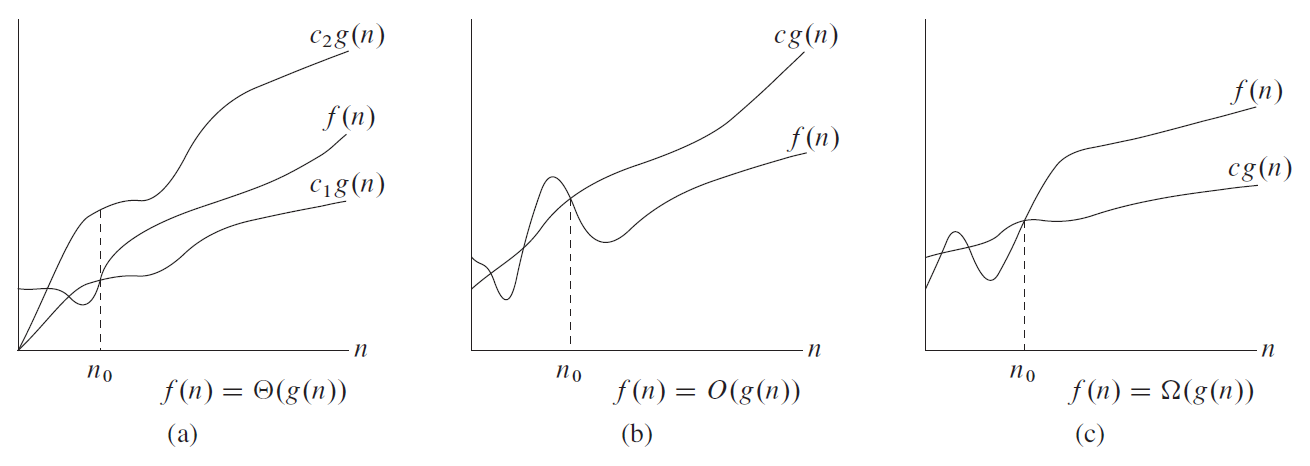
\includegraphics[width=1\textwidth]{figuras/big-o}
    \par\end{centering}
    \caption{{\small{}Ejemplos de cómo interpretar gráficamente las notaciones
    $\Theta$-grande, O-grande y $\Omega$-grande. (a) La notación $f=\Theta(g)$
    implica que la función $g$ acota $f$ tanto por arriba como por abajo;
    esto es, $g$ es una cota ajustada para $f$. (b) La notación $f=O(g)$
    implica que $g$ acota $f$ por arriba; esto es, $g$ es una cota
    superior para $f$. (c) La notación $f=\Omega(g)$ implica que $g$
    acota $f$ por abajo; esto es, $g$ es una cota inferior para $f$.}}
\end{figure}

\begin{defn}[o chica]
    Denotado como $o(g)$, es el conjunto de todas aquellas funciones
    $f$ tales que, para toda constante $c$, existe una constante $n_{0}$
    tal que $0\leq f(n)<c\cdot g(n)$ para toda $n\geq n_{0}$.
\end{defn}

\begin{defn}[$\omega$ chica]
    Denotado como $\omega(g)$, es el conjunto de todas aquellas funciones
    $f$ tales que, para toda constante $c$, existe una constante $n_{0}$
    tal que $0\leq c\cdot g(n)<f(n)$ para toda $n\geq n_{0}$.
\end{defn}

\begin{prop}
    Si $f=o(g)$, entonces $f=O(g)$.
\end{prop}

\begin{prop}
    Si $f=\omega(g)$, entonces $f=\Omega(g)$.
\end{prop}

\section{Definiciones a partir de límites}

La notación asintótica también se puede definir en términos del límite
de la razón de las funciones involucradas (suponiendo que dicho límite
existe). 

\begin{prop}
    Se tiene que
    
    \[
        \lim_{n\to\infty}\dfrac{f(n)}{g(n)}\in\begin{cases}
            [0,\infty) & \text{si y sólo si }f=O(g)\\
            (0,\infty] & \text{si y sólo si }f=\Omega(g)\\
            (0,\infty) & \text{si y sólo si }f=\Theta(g)
        \end{cases}
    \]
\end{prop}

\begin{prop}
    Se tiene que

    \[
        \text{si }\lim_{n\to\infty}\dfrac{f(n)}{g(n)}=\begin{cases}
        0 & \text{entonces }f=o(g)\\
        \infty & \text{entonces }f=\omega(g)\\
        1 & \text{entonces }f\sim g
        \end{cases}
    \]
\end{prop}

\begin{prop}
    Si $f\sim g$, entonces $f=\Theta(g)$.
\end{prop}

\section{Ordenes de crecimiento}

La notación asintótica permite clasificar las funciones según su tasa
de crecimiento. Tal clasificación se denomina \emph{orden de crecimiento}
(o, simplemente, \emph{orden}). A continuación se presentan los órdenes
de crecimiento más comunes, listados de aquél que crece más lento
al que crece más rápido.

\begin{enumerate}
    \item \emph{Constantes}: $O(1)$
    \item \emph{Logarítmicos}: $O(\log n)$
    \item \emph{Radicales}: $O(\sqrt{n})$
    \item \emph{Lineales}: $O(n)$
    \item \emph{Súper lineales}: $O(n\log n)$
    \item \emph{Cuadráticos}: $O(n^{2})$
    \item \emph{Cúbicos}: $O(n^{3})$
    \item \emph{Exponenciales}: $O(2^{n})$
    \item \emph{Factoriales}: $O(n!)$
\end{enumerate}

Se debe tener cuidado sobre cómo interpretar la lista anterior, ya
que la notación asintótica puede ocultar constantes muy grandes, lo
que puede dar una impresión equivocada de la tasa de crecimiento
de una función comparada con otra. 
Por ejemplo, supóngase que se tiene que $f(n)=10^{100}n=O(n)$
y $g(n)=10n\cdot\log n=O(n\log n)$. A pesar de que la notación
asintótica indica que $g$ crece más rápido que $f$, la realidad
es lo opuesto debido a que la constante $10^{100}$ supera por mucho 
la tasa de crecimiento de $g$.

\begin{figure}[tb]
    \begin{centering}
        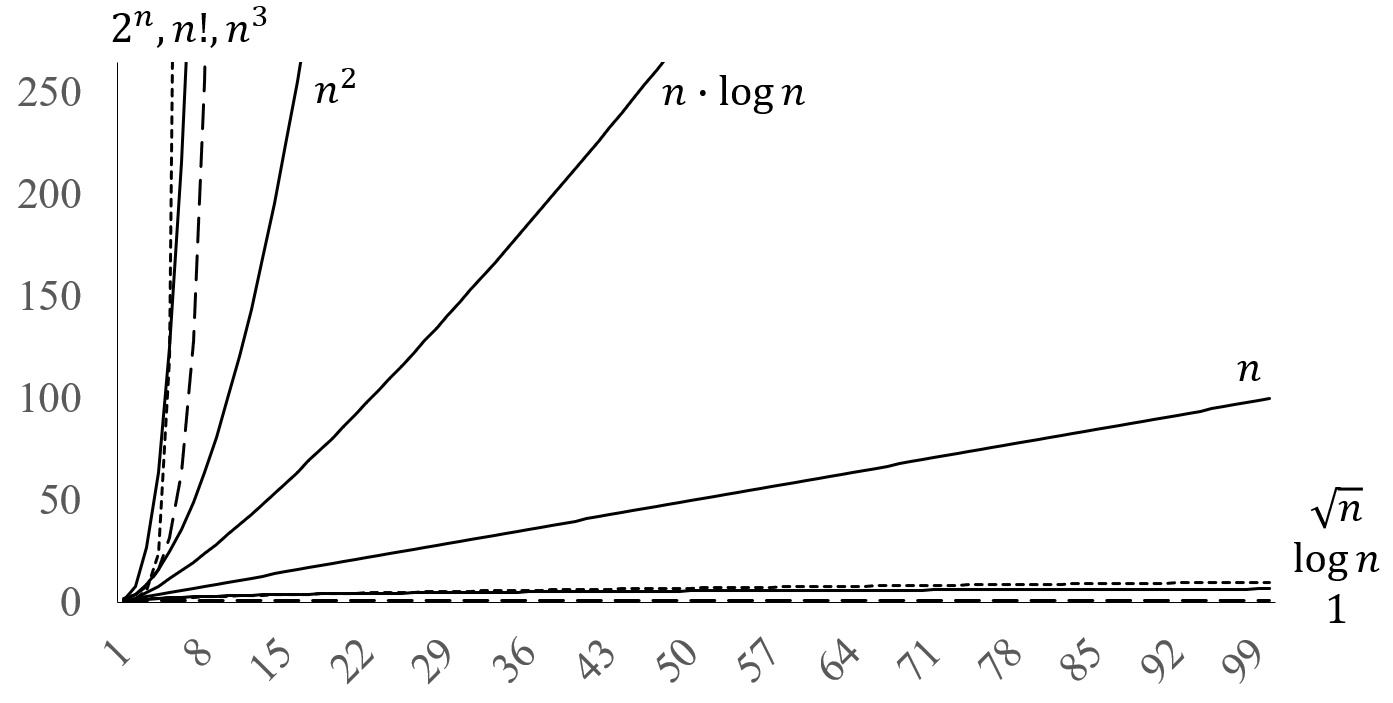
\includegraphics[width=0.8\textwidth]{figuras/ordenes}
    \par\end{centering}
    \caption{{\small{}Comparación gráfica de los órdenes de crecimiento más frecuentemente
    utilizados en las ciencias de la computación.}}
\end{figure}

\begin{thm}
    Sea $k\in\mathbb{N}_{0}$ una constante. Todo polinomio de grado $k$
    pertenece a $\Theta(n^{k})$.
\end{thm}

\begin{proof}
    Sea $f(n)=a_{k}n^{k}+a_{k-1}n^{k-1}+\dots+a_{1}n+a_{0}$ un polinomio
    arbitrario, donde $a_k,\dots,a_{0}\in\mathbb{R}$ son constantes.
    Por la definición de $\Theta$ grande, se requiere demostrar que $f=O(n^{k})$
    y que $f=\Omega(n^{k})$. 
    
    Para demostrar que $f=O(n^{k})$, se tiene que 
    
    \begin{align*}
        a_{k}n^{k}+a_{k-1}n^{k-1}+\dots+a_{1}n+a_{0} &= (a_{k}+a_{k-1}/n+\dots+a_{1}/n^{k-1}+a_{0}/n^{k})n^{k}\\
        &\leq(a_{k}+a_{k-1}+\dots+a_{1}+a_{0})n^{k}
    \end{align*}
    lo que se cumple para toda $n\geq1$. Por lo tanto, $f=O(n^{k})$.
    
    Para demostrar que $f=\Omega(n^{k})$, se tiene que 
    
    \[
        (a_{k}+a_{k-1}/n+\dots+a_{1}/n^{k-1}+a_{0}/n^{k})\cdot n^{k}\geq1\cdot n^{k}
    \]
    lo que se cumple para toda $n\geq1$. Por lo tanto, $f=\Omega(n^{k})$.
\end{proof}

\begin{thm}
    Toda función polinomial crece más rápido que cualquier función logarítmica y
    toda función exponencial crece más rápido que cualquier función polinomial.
    Esto es, sean $k,q\in\mathbb{N}$ constantes, se tiene que $(\log n)^k=o(n^q)$
    y $n^k=o([1+q]^n)$.
\end{thm}

\begin{proof}
    Ambas relaciones se pueden demostrar utilizando límites y la regla
    de L'Hopital. Así, para la primera expresión, se tiene que
    
    \begin{align*}
        \lim_{n\to\infty}\dfrac{(\ln n)^{k}}{n^{q}} &= \left(\lim_{n\to\infty}\dfrac{\ln n}{n^{q/k}}\right)^{k}\\
        &\overset{\text{H}}{=}\left(\lim_{n\to\infty}\dfrac{1/n}{(q/k)n^{q/k-1}}\right)^{k}\\
        &= \left(\lim_{n\to\infty}\dfrac{1}{(q/k)n^{q/k}}\right)^{k}\\
        &= 0
    \end{align*}
    Por lo tanto, $(\log n)^{k}=o(n^{q})$.
    
    Para la segunda expresión, se tiene que 
    
    \begin{align*}
    \lim_{n\to\infty}\dfrac{n^{k}}{(1+q)^{n}} &= \left(\lim_{n\to\infty}\dfrac{n}{(1+q)^{n/k}}\right)^{k}\\
    &\overset{\text{H}}{=}\left(\lim_{n\to\infty}\dfrac{1}{(n/k)(1+q)^{n/k-1}}\right)^{k}\\
    &= 0
    \end{align*}
    Por lo tanto, $n^{k}=o([1+q]^{n})$.
\end{proof}

\section{Propiedades aritméticas}

A continuación se describe cómo hacer aritmética con la notación asintótica.

\subsection{Adición}

La suma de las cotas de dos funciones está gobernada por la función
dominante.

\[
\begin{aligned}
    O(f)+O(g) &= O(\max\{f,g\})\\
    \Omega(f)+\Omega(g) &= \Omega(\max\{f,g\})\\
    \Theta(f)+\Theta(g) &= \Theta(\max\{f,g\})\\
    o(f)+o(g) &= o(\max\{f,g\})\\
    \omega(f)+\omega(g) &= \omega(\max\{f,g\})
\end{aligned}
\]

\subsection{Multiplicación}

La multiplicación de una función con una constante no afecta el comportamiento
asintótico de dicha función.

\[
\begin{aligned}
    O(c\cdot f) &= O(f)\\
    \Omega(c\cdot f) &= \Omega(f)\\
    \Theta(c\cdot f) &= \Theta(f)\\
    o(c\cdot f) &= o(f)\\
    \omega(c\cdot f) &= \omega(f)
\end{aligned}
\]

Cuando dos funciones se multiplican, ambas contribuyen por igual al
comportamiento asintótico de la función resultante.

\[
\begin{aligned}
    O(f)\cdot O(g) &= O(f\cdot g)\\
    \Omega(f)\cdot\Omega(g) &= \Omega(f\cdot g)\\
    \Theta(f)\cdot\Theta(g) &= \Theta(f\cdot g)\\
    o(f)\cdot o(g) &= o(f\cdot g)\\
    \omega(f)\cdot\omega(g) &= \omega(f\cdot g)
\end{aligned}
\]


\section{Comparación de funciones}

La notación asintótica se puede utilizar como un esquema para comparar
dos funciones, similar a como se puede hacer con números reales. Una
forma intuitiva de verlo es trazando las sig. analogías:

\begin{center}
\begin{tabular}{cc}
    \toprule 
        Números reales & Notación asintótica\tabularnewline
    \midrule
        $a\leq b$ & $f=O(g)$\tabularnewline
        $a\ge b$ & $f=\Omega(g)$\tabularnewline
        $a=b$ & $f=\Theta(g)$\tabularnewline
        $a<b$ & $f=o(g)$\tabularnewline
        $a>b$ & $f=\omega(g)$\tabularnewline
    \bottomrule
\end{tabular}
\par\end{center}

\subsection{Transitividad}

Sea $h:\mathbb{N}\to\mathbb{R}$ una función asintóticamente positiva. 

\begin{itemize}
    \item Si $f=\Theta(g)$ y $g=\Theta(h)$, entonces $f=\Theta(h)$.
    \item Si $f=O(g)$ y $g=O(h)$, entonces $f=O(h)$. 
    \item Si $f=\Omega(g)$ y $g=\Omega(h)$, entonces $f=\Omega(h)$.
    \item Si $f=o(g)$ y $g=o(h)$, entonces $f=o(h)$.
    \item Si $f=\omega(g)$ y $g=\omega(h)$, entonces $f=\omega(h)$.
\end{itemize}

\subsection{Reflexividad}

Las sig. igualdades se satisfacen porque $f(n)=f(n)$ para toda $n$:

\[
    \begin{aligned}
        f &= \Theta(f)\\
        f &= O(f)\\
        f &= \Omega(f)
    \end{aligned}
\]


\subsection{Simetría y simetría traspuesta}

\begin{itemize}
    \item $f=\Theta(g)$ si y sólo si $g=\Theta(f)$.
    \item $f=O(g)$ si y sólo si $g=\Omega(f)$.
    \item $f=o(g)$ si y sólo si $g=\omega(f)$.
\end{itemize}

\subsection{Carencia de tricotomía}

La tricotomía es la propiedad de los números reales donde, dados dos
números $a$ y $b$, siempre se cumple exactamente una de las sig.
condiciones: $a<b$, $a=b$ o $a>b$. La notación asintótica carece
de esta propiedad, pues se puede dar el caso donde no se cumple
que $f=O(g)$ ni que $f=\Omega(g)$. Por ejemplo, si $f(n)$ oscila
periódicamente en lugar de siempre mantener una tendencia a la alza
o a la baja.

\section*{Notas bibliográficas}

\begin{itemize}
    \item \textcite{cormen_introduction_2009}, págs. 43-52.
    \item \textcite{skiena_algorithm_2011}, págs. 34-41.
    \item \textcite{goodrich_algorithm_2001}, págs. 13-20.
    \item \href{https://www.cs.sfu.ca/~ggbaker/zju/math/growth.html}{https://www.cs.sfu.ca/$\sim$ggbaker/zju/math/growth.html}
    \item \href{http://web.mit.edu/broder/Public/asymptotics-cheatsheet.pdf}{http://web.mit.edu/broder/Public/asymptotics-cheatsheet.pdf}
    \item \href{https://people.csail.mit.edu/alinush/6.006-spring-2014/big-oh-with-limits.pdf}{https://people.csail.mit.edu/alinush/6.006-spring-2014/big-oh-with-limits.pdf}
\end{itemize}

  % \chapter{Análisis de la Eficiencia de un Algoritmo}

Después de demostrar que un algoritmo es correcto, el sig. paso es
caracterizar su tiempo de ejecución. El procedimiento que se sigue
para realizar esta tarea se denomina \emph{análisis de la eficiencia 
de un algoritmo}. En este contexto, el tiempo de ejecución de
un algoritmo se mide como la cantidad total de instrucciones que se
ejecutan. 

\section{El modelo de cómputo RAM}

Un \emph{modelo de cómputo} (model of computation) es una
representación simplificada de alguna tecnología de cómputo particular
que funge como una ``máquina abstracta'' donde se puede simular
la ejecución de un algoritmo para llevar a cabo su análisis. El modelo
debe ser lo suficientemente simple para facilitar el análisis y lo
suficientemente cercano a la tecnología que representa para que refleje
lo más fielmente posible el comportamiento que tendría el algoritmo
de ser implementado en dicha tecnología. 

Existen varios modelos de cómputo, pero el más utilizado para analizar
algoritmos secuenciales es el \emph{modelo RAM }(random access machine). 

El modelo RAM simula la arquitectura de von Neumann, la cual consiste
de una unidad de procesamiento central conectada por algún medio a
una unidad de memoria de acceso aleatorio. Esta arquitectura se caracteriza
en que las instrucciones de un programa particular y los datos del
mismo se almacenan en la misma unidad memoria y se transmiten al procesador
utilizando el mismo medio. Como consecuencia, no se puede ejecutar
una instrucción al mismo tiempo que se lee o se escribe un dato en
memoria. Estas mismas características también aplican para el modelo
RAM.

El ciclo de máquina del modelo RAM consiste de tres pasos: 

\begin{enumerate}
    \item Se lee algún dato de la memoria. 
    \item Se ejecuta alguna instrucción sobre ése dato.
    \item Se escribe el resultado en la memoria. 
\end{enumerate}

Cada ciclo de máquina se ejecuta en tiempo constante (i.e. independiente
del valor o tamaño del dato de entrada). 

En términos prácticos, al simular la ejecución de un algoritmo en
el modelo RAM, se deben seguir las sig. suposiciones:

\begin{itemize}
    \item Las instrucciones se pueden ejecutar únicamente de forma secuencial. 
    \item Todas las operaciones lógicas, aritméticas y de comparación se ejecutan
    en tiempo constante, con la excepción del exponente, el factorial,
    la raíz y el logaritmo.
    \item Se cuenta con una cantidad infinita de memoria. 
    \item Todas las operaciones de memoria (ya sea por puntero, índice o variable)
    se ejecutan en tiempo constante; no se hace distinción entre si un
    dato se encuentra en memoria caché, en la memoria RAM, en el disco
    duro, etc. 
    \item Invocar una sub-rutina toma tiempo constante, pero el tiempo requerido
    para ejecutarla depende del tamaño de su entrada.
\end{itemize}

\section{Casos a considerar}

Las clases de entrada de un algoritmo pueden categorizarse en tres
casos diferentes, dependiendo de cómo influyen en el tiempo de ejecución
de dicho algoritmo:

\begin{itemize}
    \item \emph{Mejor caso}: son todos los casos específicos que provocan que
    el algoritmo ejecute la menor cantidad de instrucciones posible. 
    \item \emph{Peor caso}: son todos los casos específicos que provocan que
    el algoritmo ejecute la mayor cantidad de instrucciones posible. 
    \item \emph{Caso promedio}: representa la cantidad promedio de instrucciones
    que el algoritmo realiza para todas las clases de entrada posibles. 
\end{itemize}

En la práctica, se suele estudiar únicamente el peor caso. En ocasiones
también se estudia el caso promedio; e.g. cuando dicho caso
ocurre con mayor frecuencia que los demás o cuando se está analizando
un algoritmo aleatorio. 

\section{Procedimiento general del análisis}

El análisis de la eficiencia de un algoritmo consiste de multiplicar
el tiempo de ejecución de cada instrucción (suponiendo que se ejecuta
en el modelo RAM) por el número de veces que se ejecuta (dada una
entrada genérica de tamaño arbitrariamente grande y perteneciente
a alguna de las clases de entrada identificadas). Al final, se suman
estos productos. 

Como resultado final del análisis, se obtiene una función $T:\mathbb{N}\to\mathbb{N}$
que caracteriza el número total de instrucciones que el algoritmo ejecuta
en proporción al tamaño de la entrada $n\in\mathbb{N}$. Esta función
se expresa por medio de su orden de crecimiento y se puede suponer
sin pérdida de generalidad que es asintóticamente positiva. 

Cabe mencionar que el significado de ``tamaño de la entrada'' depende
del contexto del problema que se está tratando. Por ejemplo, $n$
podría referirse a la longitud de un arreglo, al número de vértices
en un grafo, al valor de entrada de una función, etc.

\section*{Notas bibliográficas}

Material consultado:
\begin{itemize}
    \item \textcite{cormen_introduction_2009}, págs. 23-29.
    \item \textcite{skiena_algorithm_2012}, págs. 31-34.
    \item \textcite{goodrich_algorithm_2001}, págs. 5-6, 9-11.
\end{itemize}

  % \chapter{Relaciones de Recurrencia}

Una \emph{relación de recurrencia} (o, simplemente, \emph{recurrencia})
es una función expresada en términos de sí misma, pero con una entrada
más pequeña. Las recurrencias se presentan al analizar la
eficiencia de algoritmos de tipo \emph{divide y vencerás}. La \emph{forma
cerrada} de una recurrencia es una función equivalente, pero expresada
sin recursividad. \emph{Resolver} una recurrencia implica encontrar
su forma cerrada.

En el contexto de los algoritmos divide y vencerás, las recurrencias
suelen tener la sig. forma general: 

\[
    T(n)=\begin{cases}
        \sum_{i=1}^{p}T(n_{i})+f(n) & \text{para }n>b\\
        g(n) & \text{en caso contrario}
    \end{cases}
\]
donde

\begin{itemize}
    \item $b\in\mathbb{N}$ es la condición de paro (boundary condition); esto
    es, el valor que debe tener $n$ para entrar al caso base, 
    \item $g:\mathbb{N}\to\mathbb{N}$ es el tiempo de ejecución del caso base, 
    \item $p\in\mathbb{N}$ es la cantidad de subproblemas en las que se dividió
    la entrada, 
    \item $n_{i}\in\mathbb{N}$, tal que $n_{i}<n$, es el tamaño de la entrada
    para el subproblema $i$, 
    \item $f:\mathbb{N}\to\mathbb{N}$ es el tiempo de ejecución para dividir
    la entrada en, y/o combinar las soluciones de los, $p$ subproblemas 
\end{itemize}
La función $g$ suele omitirse cuando es constante. 

A continuación se presentan tres métodos diferentes para resolver
recurrencias.

\section{El método maestro}

El método maestro consiste simplemente en aplicar el sig. teorema.

\begin{thm}[Teorema maestro]
    Sean $a,n\in\mathbb{N}$ y $b\in\mathbb{R}$, donde $a$ y $b$ son
    constantes y $b>1$. Sea $f:\mathbb{N}\to\mathbb{N}$ una función
    asintóticamente positiva y sea $c=\log_{b}a$. Si $T:\mathbb{N}\to\mathbb{N}$
    es una recurrencia de la forma $T(n)=aT(n/b)+f(n)$, entonces se puede
    resolver de las sig. maneras:
    \begin{enumerate}
        \item Si $f=O(n^{c-\varepsilon})$ para alguna constante real $\varepsilon>0$,
        entonces $T=\Theta(n^{c})$.
        \item Si $f=\Theta(n^{c})$, entonces $T=\Theta(n^{c}\log n)$.
        \item Si $f=\Omega(n^{c+\varepsilon})$ y si, además, $af(n/b)\leq kf(n)$
        para alguna constante real $k<1$ y para todo valor de $n$ pasado
        algún umbral, entonces $T=\Theta(f)$.
    \end{enumerate}
\end{thm}

\begin{rem}
    Para el Teorema Maestro, el término $n/b$ también se puede interpretar
    como $\lceil n/b\rceil$ o $\lfloor n/b\rfloor$.
\end{rem}

La principal desventaja del Teorema Maestro es que no puede aplicarse
a cualquier tipo de recurrencia.

\section{El método del árbol recursivo}

El método del árbol recursivo es un método gráfico e informal que
consiste de construir un árbol donde cada sub-árbol representa el
tiempo requerido para resolver un subproblema en la recurrencia. Al
sumar el tiempo total de cada nivel del árbol se obtiene la forma
cerrada. 

Antes de estudiar el método en sí, es importante recordar las sig.
propiedades de los árboles $k$-arios.

\begin{prop}
    Sea $k\in\mathbb{N}_{0}$ y $n\in\mathbb{N}$. La altura de un árbol
    $k$-ario de $n$ nodos se calcula como $\lfloor\log_{k}n\rfloor+1$.
\end{prop}

\begin{prop}
    Sea $i\in\mathbb{N}_{0}$. Suponiendo que la raíz de un árbol $k$-ario
    completo se encuentra en el nivel 0, la cantidad de nodos en el nivel
    $i$, se calcula como $k^{i}$.
\end{prop}

El método del árbol recursivo consiste de los sig. pasos:

\begin{enumerate}
    \item Desglozar la recurrencia en un árbol de tal forma que la raíz represente
    el tiempo requerido para combinar y/o dividir el problema original,
    cada nodo interno represente el tiempo requerido para combinar y/o
    dividir un subproblema y cada hoja represente el tiempo requerido
    por el caso base. 
    \item Calcular la altura del árbol.
    \item Calcular la cantidad de hojas.
    \item Para cada nivel, sumar el tiempo de ejecución de todos sus nodos. 
    \item Sumar el tiempo de ejecución de todos los niveles para obtener la
    forma cerrada.
\end{enumerate}

\section{El método de sustitución}

El método de sustitución es un método formal que consiste en resolver
una recurrencia por inducción matemática. Específicamente, este método
consiste de los sig. pasos:

\begin{enumerate}
    \item Proponer una cota asintótica como la solución tentativa
    para la recurrencia.
    \item Utilizar inducción matemática para demostrar que la cota propuesta
    es correcta y para encontrar las constantes de dicha cota.
\end{enumerate}

Este método se puede utilizar para calcular tanto una cota superior
como una inferior. A continuación se presentan algunas consideraciones
y consejos que se deben tener en cuenta al trabajar con este método. 

\begin{itemize}
    \item Para proponer una buena solución tentativa:
    \begin{itemize}
        \item Se puede utilizar el método del árbol recursivo para obtener una solución
        tentativa y después utilizar el método de sustitución para demostrar
        que dicha solución es correcta o para ajustar la cota.
        \item Si la recurrencia tiene una forma similar a alguna cuya solución ya
        se conoce, se puede proponer esa solución como tentativa.
        \item Se pueden proponer dos cotas holgadas, una inferior y una superior,
        y ajustarlas gradualmente hasta que converjan en la solución correcta. 
    \end{itemize}
    \item Diferencias con la inducción matemática:
    \begin{itemize}
        \item El caso base se realiza hasta el último.
        \item La hipótesis inductiva consiste de suponer que la cota se cumple para
        $T(n_{i})$.
        \item El paso inductivo consiste en sustituir $T(n_{i})$, en la recurrencia
        original, por la forma exacta de la cota de la hipótesis inductiva.
        Este paso da origen al nombre del método.
    \end{itemize}
    \item Se debe demostrar algebraicamente que la cota propuesta se cumple
    de forma exacta. Es incorrecto aplicar la notación asintótica en el
    paso inductivo para deshacerse de constantes o términos problemáticos.
    \item Cuando la cota popuesta es lo más ajustada posible, pero aún así la
    inducción no converge, en lugar de proponer una cota más holgada,
    se puede proponer una nueva hipótesis inductiva cuya única diferencia
    con la anterior es que se le restan los términos de menor grado.
\end{itemize}

\section{Cambio de variable}

En ocasiones, se puede aplicar álgebra para transformar una recurrencia
en alguna otra cuya solución ya se conozca, eliminando
la necesidad de recurrir a cualquiera de los métodos anteriores.

\section*{Notas bibliográficas}

En las págs. 97-106 del libro de \textcite{cormen_introduction_2009} se
proporciona la demostración del Teorema Maestro. 

En las págs. 112 y 113
se proporcionan referencias a otros métodos que existen para resolver 
diferentes tipos
de recurrencias. Uno de los cuáles es el método de Akra-Bazzi, el cual
es una generalización del Teorema Maestro que admite variables contínuas
y permite resolver recurrencias donde los subproblemas varían substancialmente
de tamaño. El método de \textcite{drmota_master_2013} es una extensión
del método de Akra-Bazzi para trabajar con variables discretas. 

\begin{itemize}
    \item \textcite{cormen_introduction_2009}, págs. 83-106 y 112-113.
    \item \textcite{akra_solution_1998}.
    \item \textcite{drmota_master_2013}.
    \item \textcite{goodrich_algorithm_2001}, pág. 12.
\end{itemize}

  
  \appendix
    % \chapter{Redacción Matemática}

A diferencia de otras áreas de la ciencia, el estudio de las matemáticas
no se dedica a la recolección de evidencia física, sino a la manipulación
de conceptos abstractos y la presentación de argumentos lógicos. Es
por ello que es de suma importancia desarrollar la habilidad de buena
redacción en esta área (y, por extensión, en las ciencias de la 
computación). A continuación se proporcionan algunos consejos sobre cómo 
redactar correctamente ``trabajos matemáticos''
(i.e. artículos, reportes, ensayos, tareas, etc.).

\section{Organización del contenido}

Antes de comenzar a elaborar un trabajo escrito, es recomendable preparar
lo sig.:

\begin{itemize}
    \item Los antecedentes y la motivación del trabajo.
    \item Las definiciones y la notación a ser utilizadas.
    \item Los ejemplos a ser incluidos.
    \item Los resultados a ser presentados con sus demostraciones correspondientes
    (posiblemente en borrador). 
    \item Referencias a otros resultados que se pretenden utilizar.
    \item El orden en que todo lo anterior será presentado.
\end{itemize}

Si se prepara de antemano esta información, es más fácil escribir
el trabajo, pues sólo se requiere seguir el plan trazado.

\section{Uso apropiado de símbolos}

\begin{itemize}
    \item Nunca se debe iniciar una oración con un símbolo o una ecuación; es 
    preferible iniciar con un sustantivo seguido del símbolo que se pretende utilizar.
    Por ejemplo, en lugar de escribir:
    
    \[
        \pi\text{ es un número irracional.}
    \]
        
    es preferible escribir:
    
    \[
        \text{La constante }\pi\text{ es un número irracional.}
    \]
    
    \item De ser posible, se deben utilizar palabras en lugar de comas para separar
    aquellos símbolos que no conformen una lista. Por ejemplo, en lugar
    de escribir:
    
    \[
        \text{Al igual que }\pi\text{, }e\text{ es un número irracional.}
    \]
        
    es preferible escribir:
    
    \[
        \text{Al igual que }\pi\text{, la constante }e\text{ es un número irracional.}
    \]

    \item Se debe evitar el uso de símbolos lógicos (como $\forall$,
    $\exists$, $\Rightarrow$, i.a.) si el tema que se está tratando no
    pertenece al área de la lógica. Estos símbolos se utilizan comúnmente 
    para sustituir frases matemáticas de uso frecuente. Esta práctica es 
    aceptable si se está trabajando en un borrador o se están tomando apuntes. 
    Sin embargo, cuando se trata de trabajos formales o profesionales, 
    esta práctica debe evitarse.

    \item Se debe evitar el uso de las abreviaciones ``i.e.'' y ``e.g.''
    si se están utilizando símbolos parecidos. Si no se tiene cuidado de cómo 
    se utilizan, pueden hacer confusa la redacción. Por ejemplo, 
    en lugar de escribir ``las expresiones
    $\sqrt{-1}$ y $\lim_{n\to\infty}\left(1+1/n\right)^{n}$ no son números
    racionales; i.e. $i$ y $e$ son irracionales'' es preferible escribir:
    ``las expresiones $\sqrt{-1}$ y $\lim_{n\to\infty}\left(1+1/n\right)^{n}$
    no son números racionales; esto es, las constantes $i$ y $e$ son
    irracionales''.

    \item Todo número utilizado como un cuantificador se debe escribir con letra.
    Por ejemplo, es preferible escribir:
    
    \[
        \text{Hay exactamente dos grupos de orden 4.}
    \]
    \[
        \text{Cincuenta millones de personas no pueden estar equivocadas.}
    \]
    \[
        \text{Hay un millón de enteros positivos menores a 1,000,001.}
    \]
    
    \item No se deben mezclar símbolos con palabras en una misma oración. Por
    ejemplo, en lugar de escribir:
    
    \[
        \text{Todo entero }>1\text{ es primo o compuesto.}
    \]
    
    es preferible escribir:
    
    \[
        \text{Todo entero que mayor a 1 es primo o compuesto.}
    \]

    Otro ejemplo; aunque la sig. oración puede sonar correcta, está mal
    redactada:
    
    \[
        \text{Como }(x-2)(x-3)=0\text{, se tiene que }x=2\text{ o }3.
    \]
    
    En este caso, es preferible escribir:
    
    \[
        \text{Como }(x-2)(x-3)=0\text{, se tiene que }x=2\text{ o }x=3.
    \]

    \item No se deben introducir símbolos si no se van a utilizar. Por ejemplo,
    en la oración ``toda función biyectiva $f$ tiene una inversa'',
    si el símbolo $f$ no se vuelve a utilizar en el texto, entonces
    es preferible omitirlo. 

    \item No se deben usar símbolos sin primero haberlos introducido. Por ejemplo,
    si se tiene la expresión $n=2k+1$ y esta es la primera vez que aparece
    el símbolo $k$, entonces es preferible redactar esta expresión como:
    
    \[
        \text{Sea }k\text{ un entero, se tiene que }n=2k+1.
    \]
    \[
        \text{Se tiene que }n=2k+1\text{, donde }k\text{ es un entero.}
    \]
    
    \item Se deben seguir convenciones bien establecidas sobre el uso de
    algunos símbolos. Hay convenciones que se vienen utilizando en la
    literatura desde hace mucho tiempo y, debido a ello, uno debe apegarse
    a ellas. Algunas de estas convenciones son:

    \begin{itemize}
        \item Las letras $a$, $b$ y $c$ representan constantes. 
        \item Las letras $x$, $y$ y $z$ representan variables. 
        \item Las letras $m$ y $n$ representan enteros. 
        \item Las letras $i$ y $j$ representan índices.
        \item Las letras $f$, $g$ y $h$ representan funciones. 
        \item Las letras $u$, $v$ y $w$ representan vectores. 
        \item Las letras mayúsculas representan conjuntos o matrices.
    \end{itemize}
    
    \item Se deben utilizar parejas apropiadas de símbolos. Por ejemplo, usar
    $a$ junto con $b$ o utilizar $p$ junto con $q$, etc.

\end{itemize}

\section{Escritura de expresiones algebraicas}

Como regla general, si una expresión algebraica es relativamente corta,
entonces se puede escribir en el mismo renglón que el resto del texto.
De lo contrario, es preferible dedicarles su propio renglón, para evitar 
que una expresión larga tenga que separarse en dos renglones. 
Por otro lado, en el caso de manipulaciones algebraicas extensas, es 
recomendable saltar de renglón cada vez que se introduce
un símbolo de comparación. También es recomendable alinear todos los
símbolos de comparación en una misma columna. Por último, en aquellos
casos donde sea inevitable separar una expresión en dos renglones, es 
preferible hacerlo de tal forma que el primer renglón termine con un 
símbolo de operación y el siguiente comience con un término. De esta forma,
queda claro para el lector que la expresión en el primer renglón
está incompleta y continúa en el siguiente. 

\section{Uso apropiado de frases comunes}

\begin{itemize}

    \item Se debe utilizar el artículo ``se'' en lugar de los pronombres ``yo'',
    ``nosotros'' y ``uno''. Usar ``yo'' se considera egocéntrico,
    a menos que se hable sobre alguna experiencia personal. Usar ``nosotros''
    es adecuado, pero se corre el riesgo de sonar demasiado informal. El
    uso de ``uno'' es posible e incluso preferible en algunos casos,
    pero en otros puede ser incorrecto. El uso del artículo ``se'', seguido
    de un verbo conjugado adecuadamente, es una forma de redacción 
    muy flexible y por eso se recomienda su uso sobre los pronombres. 
    Por ejemplo, considere las sig. oraciones y compare cuál suena más apropiado:
    
    \begin{itemize}
        \item Ahora demostraré que $n$ es par.
        \item Ahora demostraremos que $n$ es par.
        \item Ahora uno demostrará que $n$ es par.
        \item Ahora se demostrará que $n$ es par.
    \end{itemize}
    
    \item Se debe evitar el uso de palabras como ``claramente'', ``obviamente'',
    ``trivialmente'', i.a. Al usar estas frases, 
    se corre el riesgo de que lo que se describe a continuación no quede 
    absolutamente claro para el lector, en cuyo caso se dejaría una mala impresión
    sobre el dominio del tema o una mala experiencia de lectura.
    
    \item Se debe tener cuidado de cómo se utilizan las frases ``para cualquier'',
    ``para algún'' y ``para todo''. Estas frases se consideran como
    equivalentes en la redacción matemática pero, si no se tiene
    cuidado del contexto en que se usan, pueden resultar en ambigüedades.
    Por ejemplo, considere la sig. oración: ``Se dice que el conjunto
    $S$ satisface la propiedad $P$ si $P$ se satisface para cualquier
    elemento $s\in S$''. En este caso, queda ambigüo si la propiedad
    $P$ se debe cumplir para todos los elementos de $S$ o solamente
    para uno. En situaciones como esta, es preferible evitar completamente
    la frase ``para cualquier'' en favor de una redacción más explícita;
    e.g. utilizando frases como ``para todo/cada'', ``para algún''
    o ``para al menos uno''.
    
    \item Es incorrecto utilizar la palabra ``como'' en conjunto con ``entonces''.
    Por ejemplo, en lugar de escribir:
    
    \[
        \text{Como }n^{2}\text{ es par, entonces }n\text{ también es par.}
    \]
    
    es preferible escribir cualquiera de estas:

    \[
        \text{Si }n^{2}\text{ es par, entonces }n\text{ también es par.}
    \]
    \[
        \text{Como }n^{2}\text{ es par, se tiene que }n\text{ también es par.}
    \]
    \[
        \text{Como }n^{2}\text{ es par, }n\text{ también es par.}
    \]
    
    \item No se debe utilizar en cantidades abusivas frases como ``por lo tanto'',
    ``lo que implica'', ``como consecuencia'', etc. El propósito de
    estas frases es encadenar varios razonamientos para formar un
    argumento lógico. Utilizar la misma frase de forma repetitiva
    puede volverse muy tedioso para el lector. Debido a ello, se recomienda 
    utilizar una variedad más amplia de frases y, por lo menos, se debe evitar 
    utilizar la misma frase dos veces seguidas. Naturalmente, esto requiere de 
    creatividad y práctica.

\end{itemize}

\section{Consejos generales}

\begin{itemize}
    \item Se deben escribir oraciones completas y que sean gramatical y ortográficamente
    correctas. Se sugiere conjugar igual todos los verbos de una misma oración y utilizar
    conjugaciones simples siempre que sea posible. 
    \item La escritura es un proceso iterativo; rara vez se puede escribir algo
    correctamente en el primer intento. Es por ello que se recomienda
    releer \emph{desde el principio} el trabajo que se está escribiendo
    cada vez que se le hace alguna corrección. También es recomendable
    dejar descansar el escrito unos días antes de volver a revisarlo. 
    \item A la hora de escribir, se debe considerar la audiencia para la que
    se está escribiendo; esto es, se debe elegir el vocabulario y estilo
    de redacción adecuados para ella y se debe considerar su conocimiento
    previo al decidir cuánta información incluir y cuánta omitir. 
    \item Nunca se debe entregar o publicar un trabajo escrito sin antes permitir
    que alguien más lo lea y proporcione retroalimentación. Además, toda
    corrección realizada al escrito debe ser verificada por la misma persona
    que sugirió dicha corrección.
\end{itemize}

\section*{Notas bibliográficas}

\begin{itemize}
    \item \textcite{chartrand_mathematical_2012}, págs. 1-13.
\end{itemize}
%% mover a matematicas discretas
    \chapter{La potencia}

Sea \(x\in\mathbb{R}\) distinto de cero y denominado \emph{base} y sea \(n\in\mathbb{N}\) denominado \emph{exponente}. 
La \emph{n-ésima potencia} de \(x\), denotada como \(x^n\), es el producto de \(n\) bases \(x\); esto es, \(x^n\triangleq x\cdot x\cdot\dots(n\text{ veces})\).

\section{Leyes de los exponentes}

Sean \(x,y\in\mathbb{R}\) distintos de cero y sean \(m,n\in\mathbb{N}\).
Se tienen las sig. identidades:
\begin{enumerate}
  \begin{multicols}{3}
    \item \(x^{0}\triangleq1\)
    \item \(x^{1}\triangleq x\)
    \item \(x^{-1}\triangleq1/x\)
    \item \(x^{m/n}\triangleq\sqrt[n]{x^{m}}\)
    \item \(x^{m}x^{n}=x^{m+n}\)
    \item \(x^{m}/x^{n}=x^{m-n}\)
    \item \((x^{m})^{n}=x^{mn}\)
    \item \((xy)^{n}=x^{n}y^{n}\)
    \item \((x/y)^{n}=x^{n}/y^{n}\)
  \end{multicols}
\end{enumerate}

Las identidades anteriores se justifican de las sig. manipulaciones algebraicas:

\begin{flalign}\tag{5}
  x^mx^n &= x\cdot x\cdot\dots (m\text{ veces})\cdot x\cdot x\dots (n\text{ veces}) &&\\
  &= x^{m+n}\nonumber
\end{flalign}

\begin{flalign}\tag{6}
  \text{\textit{Caso 1}} &: \text{ Si }m>n\text{, entonces} \nonumber&&\\
  x^m/x^n &= \dfrac{x\cdot x\cdot\dots (m\text{ veces})}{x\cdot x\cdot\dots (n\text{ veces})} \nonumber&&\\
  &= 1\cdot 1\cdot\dots(n\text{ veces})\cdot x\cdot x\cdot\dots(m-n\text{ veces}) \nonumber&&\\
  &=x^{m-n} \nonumber&&\\
  \text{\textit{Caso 2}} &: \text{ Si }m=n\text{, entonces} \nonumber&&\\
  x^m/x^n &=1\cdot 1\cdot\dots (m=n\text{ veces}) \nonumber&&\\
  &=x^0 \nonumber&&\\
  &=x^{m-n}\nonumber&&\\
  \text{\textit{Caso 3}} &: \text{ Si }m<n\text{, entonces} \nonumber&&\\
  x^m/x^n &=1\cdot 1\cdot\dots(m\text{ veces})\cdot 1/x\cdot 1/x\cdot\dots(n-m\text{ veces}) \nonumber&&\\
  &=1/x^{n-m} \nonumber&&\\
  &=x^{m-n} \nonumber
\end{flalign}

\begin{flalign}\tag{7}
  (x^m)^n &= [x\cdot x\cdot\dots (m\text{ veces})]\cdot[x\cdot x\cdot\dots (m\text{ veces})]\dots[n\text{ veces}] &&\\
  &= x^{mn}\nonumber
\end{flalign}

\begin{flalign}\tag{8}
  (xy)^n &= xy\cdot xy\cdot\dots (n\text{ veces}) &&\\
  &= x\cdot x\cdot\dots (n\text{ veces})\cdot y\cdot y\cdot\dots (n\text{ veces}) \nonumber&&\\
  &= x^ny^n\nonumber
\end{flalign}

\begin{flalign}\tag{9}
  (x/y)^n &= \dfrac{x}{y}\cdot\dfrac{x}{y}\cdot\dots (n\text{ veces}) &&\\
  &= x^n/y^n\nonumber
\end{flalign}

    \chapter{El logaritmo}

Sea \(x\in\mathbb{R}\) mayor a cero y denominado \emph{argumento} y sea \(b\in\mathbb{R}\) distinto de 1 y denominado \emph{base}.
El \emph{logaritmo} de \(x\) con respecto a \(b\), denotado como \(\log_{b}x\), es la potencia a la que hay que elevar \(b\) para obtener \(x\) como resultado; esto es, \(y=\log_{b}x\) si y sólo si \(b^{y}=x\), donde \(y\in\mathbb{R}\).

\begin{table}[h]
  \caption{Diferentes tipos de logaritmos, su base y su notación correspondiente.}
  \begin{center}
    \begin{tabular}{ccc}
      \toprule
      Tipo de logaritmo & Base & Notación \\
      \midrule
      Decimal & 10 & \(\log{x}\) \\
      Natural & \(e\) & \(\ln{x}\) \\
      Binario & 2 & \(\lg{x}\) \\
      \bottomrule
    \end{tabular}
  \end{center}
\end{table}

\begin{prop}
  La base de un logaritmo no puede ser 0 ni 1.
\end{prop}
  
Debido a que \(0^x=0\) para toda \(x>0\) y debido a que \(1^x=1\) para toda \(x\), los logaritmos con base 0 y 1 no tienen una solución definida.

\begin{prop}
  La base de un logaritmo no puede ser negativa.
\end{prop}

De lo contrario, dependiendo del argumento del logaritmo, la solución podría ser un número complejo.

\begin{prop}
  El argumento de un logaritmo no puede ser negativo.
\end{prop}

Debido a que todo número positivo elevado a cualquier potencia siempre resulta en un número positivo, el logaritmo (con base positiva) de un número negativo no tendría solución.

\section{Leyes de los logaritmos}

Sean \(b,v,x,y\in\mathbb{R}\), donde los valores \(x\) y \(y\) son mayores a cero y los valores \(b\) y \(v\) son distintos de 1. Se tienen las sig. identidades:

\marginnote[1\baselineskip]{La identidad 7 se conoce como la ley de cambio de base. Esta ley implica que \(\log_v{x}=\log_v{b}\cdot\log_b{x}\); esto es, para cambiar la base de un logaritmo, basta con multiplicarlo por un factor constante. Debido a esto, no importa la base de un logaritmo, su comportamiento asintótico siempre será el mismo y es por esta razón que la base del logaritmo suele omitirse al utilizar la notación asintótica.}

\begin{enumerate}
  \begin{multicols}{2}
    \item \(\log_b{1}=0\)
    \item \(\log_b{b}=1\)
    \item \(\log_b(xy)=\log_b{x}+\log_b{y}\)
    \item \(\log_b(x/y)=\log_b{x}-\log_b{y}\)
    \item \(\log_bx^y=y\log_b{x}\)
    \item \(\log_b\sqrt[y]{x}=1/y\cdot\log_b{x}\)
    \item \(\log_b{x}=\log_v{x}/\log_v{b}\)
    \item \(\log_b{x}=1/\log_x{b}\), si \(x\neq 1\)
    \item \(x^{\log_b{y}}=y^{\log_b{x}}\)
  \end{multicols}
\end{enumerate}

Las identidades anteriores se justifican de las manipulaciones algebraicas que se presentan a continuación. Considérese que \(p,q\in\mathbb{R}\) tales que \(x=b^p\) y \(y=b^q\), lo que implica que \(p=\log_b{x}\) \& \(q=\log_b{y}\) (por la definición del logaritmo):
\begin{flalign}
  \text{Es consecuencia directa del hecho que } b^0=1\text{ para cualquier }b.
\end{flalign}
\begin{flalign}
  \text{Es consecuencia directa del hecho que } b^1=b\text{ para cualquier }b.
\end{flalign}
\begin{align}
  xy &= b^pb^q &&\\
  xy &= b^{p+q} \nonumber&&\\
  \log_b(xy) &= p+q \nonumber&&\\
  \log_b(xy) &= \log_b{x}+\log_b{y} \nonumber
\end{align}
\begin{align}
  x/y &= b^p/b^q &&\\
  x/y &= b^{p-q} \nonumber&&\\
  \log_b(x/y) &= p-q \nonumber&&\\
  \log_b(x/y) &= \log_b{x}-\log_b{y} \nonumber
\end{align}
\begin{align}
  x &= b^p &&\\
  x^y &= (b^p)^y \nonumber&&\\
  x^y &= b^{py} \nonumber&&\\
  \log_b{x^y} &= py \nonumber&&\\
  \log_b{x^y} &= y\log_b{x} \nonumber
\end{align}
\begin{align}
  x &= b^p &&\\
  \sqrt[y]{x} &= \sqrt[y]{b^p} \nonumber&&\\
  \sqrt[y]{x} &= b^{p/y} \nonumber&&\\
  \log_b \sqrt[y]{x} &= p/y \nonumber&&\\
  \log_b \sqrt[y]{x} &= 1/y\cdot \log_b{x} \nonumber
\end{align}
\begin{align}
  b^p &= x &\\
  \log_v{b^p} &= \log_v{x} \nonumber&&\\
  p\log_v{b} &= \log_v{x} \nonumber&&\\
  p &= \dfrac{\log_v{x}}{\log_v{b}} \nonumber&&\\
  \log_b{x} &= \log_v{x}/\log_v{b} \nonumber
\end{align}
\begin{align}
  \log_b{x} &= \dfrac{\log_v{x}}{\log_v{b}} &&\\
  \log_b{x} &= \dfrac{\log_x{x}}{\log_x{b}} \nonumber&&\\
  \log_b{x} &= \dfrac{1}{\log_x{b}} \nonumber
\end{align}
\begin{align}
  x^{\log_b{y}}=x^q=(b^p)^q=b^{pq}=(b^q)p=y^p=y^{\log_b{x}}
\end{align}

  
  \printbibliography[heading=bibintoc]
\end{document}
